\documentclass[dvipsnames,svgnames,beamer, 12pt]{beamer}

\usetheme{Boadilla}
%\usecolortheme{seahorse}

\usepackage[utf8]{inputenc}

\usepackage{cancel}

\usepackage{lib}
\usepackage{tikz}
\usetikzlibrary{arrows.meta}
\tikzset{%
  >={Latex[width=2mm,length=2mm]},
  % Specifications for style of nodes:
            base/.style = {rectangle, rounded corners, draw=black,
                           minimum width=4cm, minimum height=1cm,
                           text centered},
         solid/.style = {base, minimum width=2.5cm, fill=cyan!10,
                           font=\ttfamily},
         invisible/.style = {},
}
\usetikzlibrary{positioning}
\usepackage{alltt}


\setbeamercovered{invisible}

\setbeamertemplate{navigation symbols}{}

\setbeamertemplate{footline}{\hfill\insertframenumber\hfill\vspace{3mm}}

\title{Extending the herd Memory model simulator}

\author{Simon Colin}

\date{\today}

\begin{document}

\begin{frame}
	\titlepage
\end{frame}

% passer regles rc11 en cat
% expliquer no thin air
% conclusion

\begin{frame}[fragile]{Memory models}

	\begin{figure}
	\centering
	\begin{tabular}{p{4cm} || p{4cm}}
	Thread 0 & Thread 1 \\
	\hline \\
	x $\leftarrow$ 1 & y $\leftarrow$ 1 \\
	r0 $\leftarrow$ y & r1 $\leftarrow$ x 
	\end{tabular}
	\end{figure}
	\vfill
	Can we have $r0 = 0$ and $r1 = 0$?
	
	We expect the instructions to be executed in order, so this shouldn't be possible.
	
	On modern processors, this behaviour can happen.

\end{frame}

\begin{frame}[fragile]{Memory events}

	Programs are made of instructions.
	\vfill 
	Instructions involve memory events : reads from and writes to the shared memory.
	\vfill
	\begin{figure}
	\centering
	\begin{tabular}{p{4cm} p{4cm}}
	Instructions & Events \\
	\begin{verbatim}
	x = 1;
	a = x;
	fence;
	y++;
	\end{verbatim} &
	\begin{verbatim}
	Store(x, 1)
	Read(x)
	Fence
	Read(y, s0)
	Store(y, s0 + 1)
	\end{verbatim} \\
	\end{tabular}
	\end{figure}
	$x$ and $y$ are shared variables, $a$ is a local variable
	\vfill

\end{frame}

\begin{frame}{A simple model : sequential consistency}

	Two properties :
	\begin{itemize}
	\item No local reordering : the events occur in the same order as in the program.
	\item Instantaneous memory : when a thread writes to memory all threads see the value instantly.
	\end{itemize}

\end{frame}

\begin{frame}{Weaker memory models}

	\vfill
	Modern memory models allow more behaviors than sequential consistency.
	\vfill
	Such behaviours result from :\begin{itemize}
	\item out of order execution
	\item speculative execution
	\item writes don't become visible to every thread at the same time
	\end{itemize}
	\vfill
%	Fortunately, there are means to restore ordering.
%	\vfill

\end{frame}

\iffalse
\begin{frame}{Restoring ordering}

	Fences : instructions that ensure events before the fence occur before those after the fence.
	\vfill
	Data dependencies : when an instruction A uses the value of an instruction B for some calculation.
	\vfill
	In such a situation processors will ensure B occurs before A.

\end{frame}

\begin{frame}[fragile]{litmus tests}

	\vfill
	\vfill
	A litmus test is a short parallel program and an assertion about the result.
	\begin{figure}
	\centering
	\begin{tabular}{p{4cm} p{4cm}}
	\begin{verbatim}
	Thread 0
	x = 1;
	y = 1;
	\end{verbatim} &
	\begin{verbatim}
	Thread 1
	while(y = 0) {}
	r1 = x;
	\end{verbatim}
	\end{tabular}
	\centerline{Always $r1 = 1$}
	\caption{The message passing litmus test}
	\end{figure}
	\vfill
	We use them to find out about the possible behaviours of machines.
	\vfill
	\vfill

\end{frame}\fi

\begin{frame}{Executions}

	Executions are a set of events and relations.
	\begin{figure}
	\centering
	\begin{columns}
	\begin{column}{5cm}
	\begin{figure}[b]
	\centering
	\raisebox{-\totalheight}{\includegraphics[width=4.1cm]{exec}}
	\end{figure}
	\end{column}
	\begin{column}{5cm}
	\begin{itemize}
	\item program order $\po$
	\item memory order $\mo$
	\item read from $\rf$
	\item many more relations ...
	\end{itemize}
	\end{column}
	\end{columns}
	
	\end{figure}

\end{frame}

\iffalse
\begin{frame}{RC11 : events}

	\vfill
	fences
	\vfill
	non atomic memory events
	\vfill
	atomic memory events annotated with a memory order : \begin{itemize}
	\item Relaxed
	\item Acquire
	\item Release
	\item Sequentially consistent
	\end{itemize}
	\vfill
%	data race: when two events that aren't both atomic or both reads can access the same location at the same time.
%	\vfill
%	Data races cause unspecified behaviour.

\end{frame}\fi

\begin{frame}[fragile]{RC11}

	\vfill
	An RC11\footnote{Repairing sequential consistency in C/C++11, Proceedings of the 38$^{th}$ ACM SIGPLAN Conference} consistent execution satisfies :
	\begin{itemize}
	\item \verb$irreflexive (hb; eco?)$ \hfill (coherence)
	\item \verb$empty (rmw & (rb; mo))$. \hfill (atomicity)
	\item \verb$acyclic (po | rf)$ \hfill (no-thin-air)
	\item \verb$acyclic psc$ \hfill (sequential-consistency)
	\end{itemize}
	\vfill
	

\end{frame}

\begin{frame}[fragile]{no-thin-air}

	\verb!acyclic (po | rf)!
	\vfill
	\begin{itemize}
	\item If we read from a write, the write has to have taken place first.
	\item If a write depends on a read, the read has to have taken place first.
	\end{itemize}
	
	$\dep;\rf$ causality loops are possible.
	
	Since $\dep \subseteq \po$ we forbid $\dep;\rf$ loops by simply banning $\po;\rf$ loops.

\end{frame}

\begin{frame}{Herd}
	\begin{figure}
	\centering
	{\fontsize{10pt}{0}
	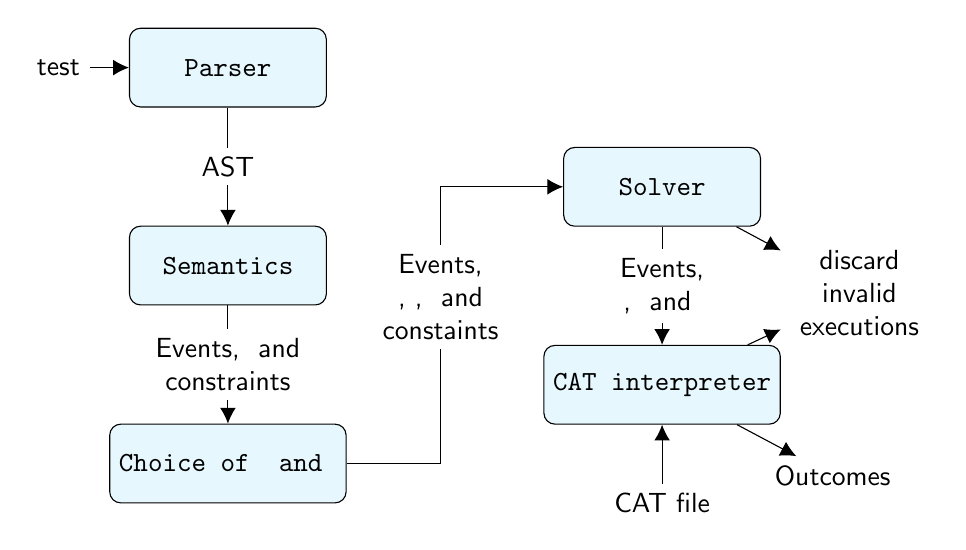
\begin{tikzpicture}[every node/.style={fill=white, font=\sffamily}, node distance=1.5cm, align=center]

	\node (start) [invisible] {test};
	\node (parser) [solid, right = 0.5cm of start] {Parser};
	\node (sem) [below = of parser, solid] {Semantics};
	\node (choice) [below = of sem, solid] {Choice of $\rf$ and $\mo$};
	\node (solver) [below right = 0.5cm and 3 of parser, solid] {Solver};
	\node (interp) [below = of solver, solid] {CAT interpreter};
	\node (end) [invisible, below right = 0.4cm and -0.2cm of interp] {Outcomes};
	\node (model) [invisible, below of = interp] {CAT file};
	\node (reject) [invisible, below right = 0.17cm and 0.25cm of solver, text width = 1.75cm] {discard invalid executions};
	
	\draw[->] (start) -- (parser);
	\draw[->] (parser) -- node {AST} (sem);
	\draw[->] (sem) -- node[text width = 2.5cm] {Events, $\po$ and constraints} (choice);
	\draw[->] (choice) -| ++(2.7,1) |- node[text width= 2cm, minimum size = 0.1cm, yshift=-1.4cm] {Events, $\po$, $\mo$, $\rf$ and constaints} (solver);
	\draw[->] (solver) -- node[text width = 2cm] {Events, $\po$, $\mo$ and $\rf$} (interp);
	\draw[->] (interp) -- (end);
	\draw[->] (model) -- (interp);
	\draw[->] (solver) -- (reject);
	\draw[->] (interp) -- (reject);
	
	\end{tikzpicture}}
	\end{figure}

\end{frame}

\begin{frame}[fragile]{Herd}

	\begin{figure}
	\centering
	\begin{lstlisting}
herd(execution $E$)
{
  forall $\mo$ on $E$
  {
    forall $\rf$ on execution $E$
    {
      if consistent(CAT model, $E$, $\mo$, $\rf$)
      then add(outcomes, $E$, $\mo$, $\rf$)
    }
  }

	\end{lstlisting}
	\end{figure}

\end{frame}

\begin{frame}{Herd}

	\vfill
	Generates every combination of $\rf$ and $\mo$, this is expensive.
	\vfill
	Dealing with large sets of executions is a common problem for model checkers.
	\vfill
	\begin{center}
	Solution : a stateless incremental algorithm\footnote{Effective stateless model checking for C/C++ concurrency, Proceedings of the ACM on Programming Languages, Colume 2 Issue POPL} that avoids building most inconsistent executions.
	\end{center}

\end{frame}

\begin{frame}{My project}

	Implement RC11 in CAT.  
	\vfill
	Implement the RC11 check directly into Herd.
	\vfill
	Implement the stateless algorithm in Herd.
%	\vfill
%	Should time allow it, I will try implementing smt based rc11 model checking techniques as well.

\end{frame}
\iffalse
\begin{frame}{The stateless algorithm}

	All RC11 properties but SC are monotonous.
	\vfill
	
	Work recursively :
	\begin{itemize}
	\item start with a consistent partial execution.
	
	\item add an event 
	
	\item call the algorithm recursively on evey possible consistent partial execution (choice of $\mo$ or $\rf$).
	\end{itemize}
\end{frame}\fi

\begin{frame}[fragile]{The stateless algorithm}

\begin{figure}
\centering
\begin{small}
\begin{lstlisting}
visit(execution $E$) {
  if has_events_to_add($E$)
  then
  {
    $e$ = next_event($E$)
    $execs$ = possible_extensions($E$, $e$)
    for $ex$ in $execs$
    {
      if rc11_consistent($ex$)
      then visit($ex$)
    }
  } else {
    if acyclic($E$.psc)
    then add(outcomes, $E$)
  }}
\end{lstlisting}
\end{small}
\end{figure}

\end{frame}

\begin{frame}{How the stateless algorithm works}

	\begin{figure}
	\centering
	{\fontsize{10pt}{0}
	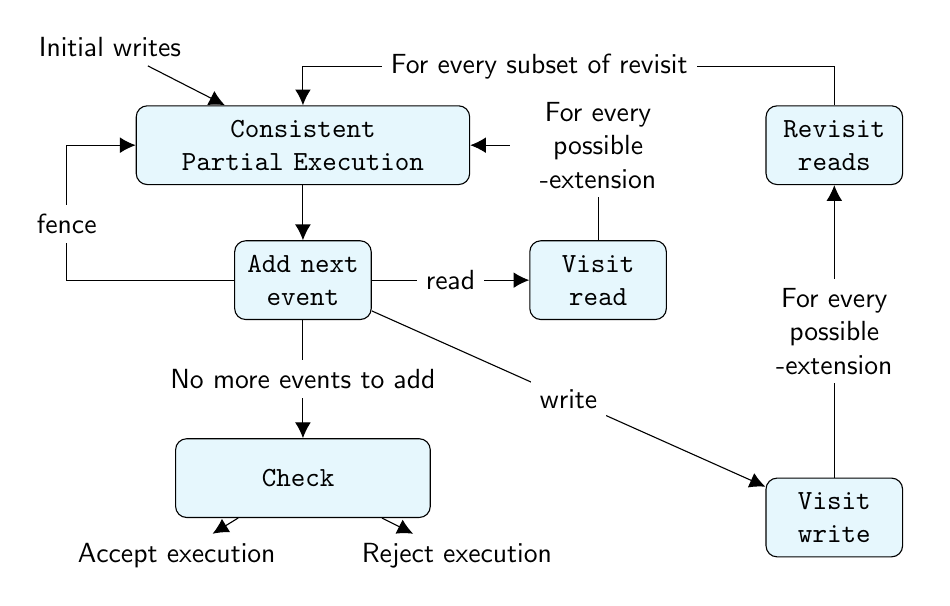
\begin{tikzpicture}[every node/.style={fill=white, font=\sffamily}, node distance=1.5cm, align=center, minimum width = 0]
	
	\node (cpe) [solid, text width = 4cm]{Consistent Partial Execution};
	\node (add) [solid, below = 0.7cm of cpe, text width = 1.5cm, minimum width = 0] {Add next event};
	\node (read) [solid, right = 2cm of add, text width = 1.5cm, minimum width = 0] {Visit read};
	\node (write) [solid, below right = 2cm and 5cm of add, text width = 1.5cm, minimum width = 0] {Visit write};
	\node (revisit) [solid, right = 3.75cm of cpe, text width = 1.5cm, minimum width = 0] {Revisit reads};
	\node (done) [solid, below = of add, text width = 3cm] {Check $\psc$};
	\node (in) [invisible, above left = 0.5cm and -0.7cm of cpe] {Initial writes};
	\node (accept) [invisible, below left = 0.2cm and -1.4cm of done] {Accept execution};
	\node (reject) [invisible, below right = 0.2cm and -1cm of done] {Reject execution};
	
	
	\draw[->] (cpe) -- (add);
	\draw[->] (add) -- node {read} (read);
	\draw[->] (add) -- node {write} (write);
	\draw[->] (add) -- node {No more events to add} (done);
	\draw[->] (add) -| ++(-3cm,0) |- node[yshift=-1cm] {fence} (cpe);
	\draw[->] (read) |- node[text width = 2cm] {For every possible $\rf$-extension} (cpe);
	\draw[->] (write) -- node [text width = 2cm]{For every possible $\mo$-extension} (revisit);
	\draw[->] (revisit) |- ++(0,1cm) -| node[xshift = 3cm] {For every subset of revisit} (cpe);
	\draw[->] (in) -- (cpe);
	\draw[->] (done) -- (accept);
	\draw[->] (done) -- (reject);
	
	\end{tikzpicture}}
	
	\end{figure}	 

\end{frame}

\iffalse \begin{frame}{Differences between the reference and my implementation}

	Herd generates a set of events and constraints per possible path.
	
	Some partial executions get computed more than once.
	\vfill
	Some parts of the reference algorithm aren't relevant to herd.

\end{frame}\fi

\begin{frame}{Conclusion}

	My algorithm works for CAS-free programs.
	
	It is faster than Herd for larger tests, but slower for shorter ones.
%	This is likely due to the smaller number of executions to discard on smaller tests.
	\vfill
	The treatment of CAS is not finished yet, this is difficult because of differences in the handling of semantics between Herd and the reference.
\end{frame}

\begin{frame}{Further work}

	\begin{itemize}
	\item finish the implementation
	\item test the incremental algorithm against the RC11 CAT file
	\item optimize the performance
	\item work on SMT-based memory model checking
	\end{itemize}

\end{frame}

\end{document}